\documentclass[11pt, a4paper]{report}

%====================== PACKAGES ======================

\usepackage[french]{babel}
\frenchbsetup{StandardLists=true}
\usepackage{enumitem}
\usepackage{pifont}
\usepackage[utf8x]{inputenc}
%pour gérer les positionnement d'images
\usepackage{float}
\usepackage{amsmath}
\DeclareMathOperator{\dt}{dt}
\usepackage{graphicx}
\usepackage{tabularx}
\usepackage[colorinlistoftodos]{todonotes}
\usepackage{url}
%pour les informations sur un document compilé en PDF et les liens externes / internes
\usepackage[pdfborder=0]{hyperref}
\hypersetup{
	colorlinks = true
	}
%pour la mise en page des tableaux
\usepackage{array}
\usepackage{tabularx}
\usepackage{multirow}
\usepackage{multicol}
%pour utiliser \floatbarrier
%\usepackage{placeins}
%\usepackage{floatrow}
%espacement entre les lignes
\usepackage{setspace}
%modifier la mise en page de l'abstract
\usepackage{abstract}
%police et mise en page (marges) du document
\usepackage[T1]{fontenc}
\usepackage[top=2cm, bottom=2cm, left=2cm, right=2cm]{geometry}
%Pour les galerie d'images
\usepackage{subfig}

\usepackage{pdfpages}

%====================== INFORMATION ET REGLES ======================

%rajouter les numérotation pour les \paragraphe et \subparagraphe
\setcounter{secnumdepth}{4}
\setcounter{tocdepth}{4}

\hypersetup{							% Information sur le document
pdfauthor = {Stephan Runigo},			% Auteurs
pdftitle = {Documentation simulateurs physiques},			% Titre du document
pdfsubject = {Documentation des simulateurs de chaine de pendules},		% Sujet
pdfkeywords = {SiCP, SiCF, chaine de pendules, corde vibrante, transformée de fourier, gaz parfait},	% Mots-clefs
pdfstartview={FitH}}	% ajuste la page à la largeur de l'écran
%pdfcreator = {MikTeX},% Logiciel qui a crée le document
%pdfproducer = {} % Société avec produit le logiciel
%======================== DEBUT DU DOCUMENT ========================
%
\begin{document}
%
%régler l'espacement entre les lignes
\newcommand{\HRule}{\rule{\linewidth}{0.5mm}}
%
%page de garde
\begin{titlepage}
\begin{center}

% Upper part of the page. The '~' is needed because only works if a paragraph has started.
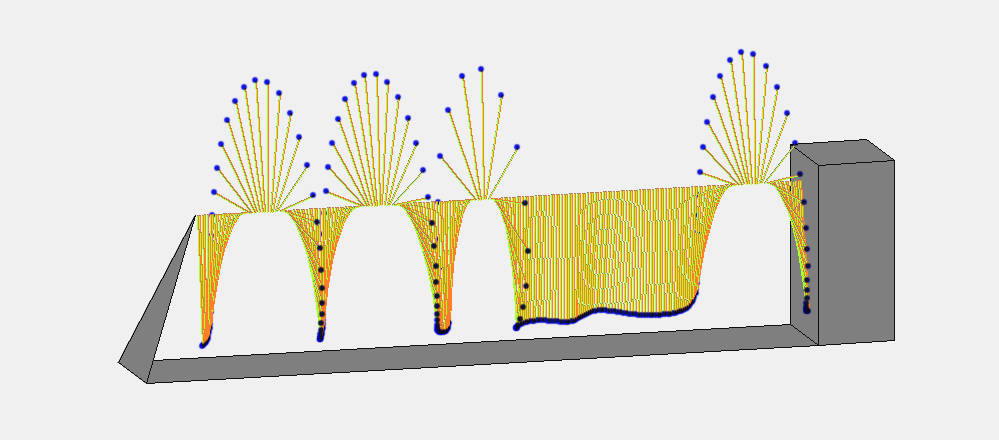
\includegraphics[width=.6\textwidth]{./illustration/SiCP2}
%\caption{SiCF}
\label{fig:image1}
~\\[1cm]

\begin{figure}[htbp]
\begin{minipage}[c]{.45\linewidth}
\begin{center}
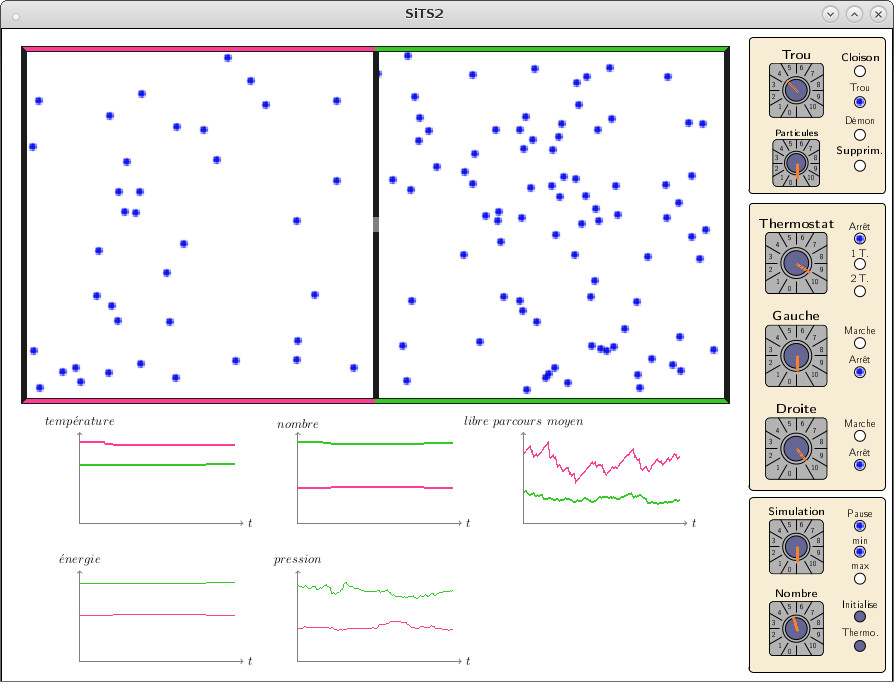
\includegraphics[scale=0.25]{./illustration/SiTS2}
%\caption{SiCF}
%\label{fig:image1}
\end{center}
\end{minipage}
\hfill
\begin{minipage}[c]{.45\linewidth}
\begin{center}
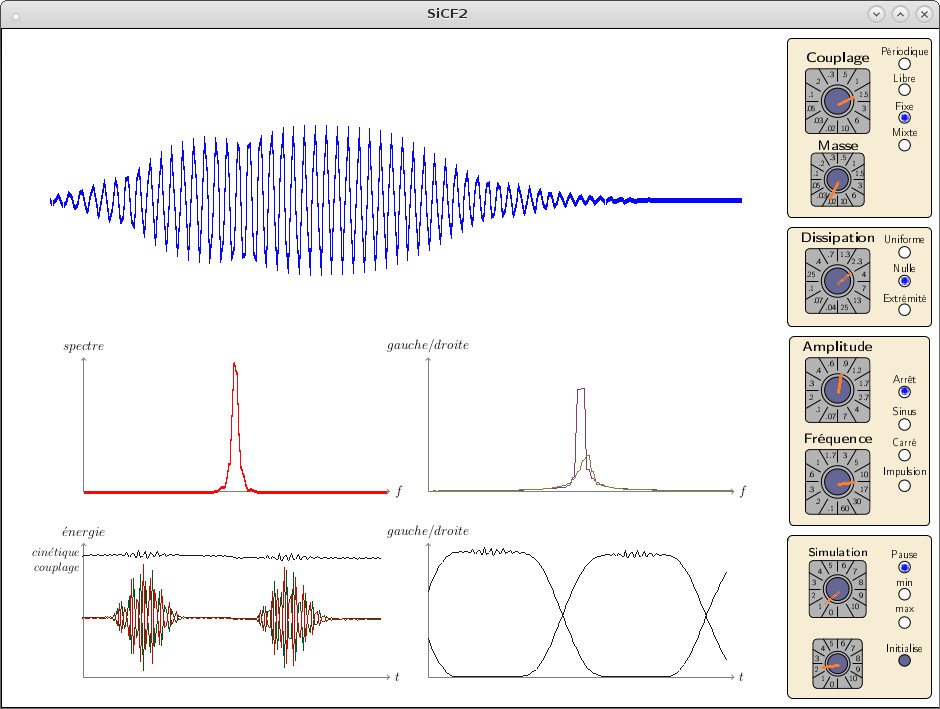
\includegraphics[scale=0.23]{./illustration/SiCF2}
%\caption{diagramme des tâches.}
%\label{SiCP}
\end{center}
\end{minipage}
\end{figure}
%\textsc{\LARGE Complément nutritionnel}\\[1.5cm]
~\\[1cm]

\textsc{\Large }\\[0.5cm]

% Title
\HRule \\[0.4cm]

{\huge \bfseries  SiCP2, SiCF2, SiTS2\\
Documentation et théorie\\[0.4cm] }

\HRule \\[1.5cm]

% Author and supervisor
\begin{minipage}{0.4\textwidth}
\begin{flushleft} \large
%\emph{Auteur:}\\
%Stephan \textsc{Runigo}
\end{flushleft}
\end{minipage}
\begin{minipage}{0.4\textwidth}
\begin{flushright} \large
\emph{Auteur:}\\
Stephan \textsc{Runigo}
\end{flushright}
\end{minipage}

\vfill

% Bottom of the page
{\large \today}

\end{center}
\end{titlepage}

%
%page blanche
\begin{center}
\Large
Résumé
\normalsize
\end{center}
\vspace{3cm}
\begin{itemize}[leftmargin=1cm, label=\ding{32}, itemsep=21pt]
\item {\bf Objet : }Ce document (en cours de construction), accompagne les programmes SiCP, SiCF et SiGP (eux mêmes en cours de développement).
\item {\bf Contenu : }Il contient un manuel d'installation et d'utilisation ainsi que quelques développements théoriques liés à ces programmes de simulations numériques.
\item {\bf Public concerné : }Ce document s'adresse aux enseignants et aux étudiants du supérieur des sections sciences physiques et informatique.
\end{itemize}

\vspace{3cm}

SiCP, SiCF et SiGP sont des simulateurs numériques d'équations physiques offrant une représentation graphique et une interaction dynamique avec les paramètres physiques. Destinés à un usage pédagogique, ils permettent de visualiser le comportement des systèmes physiques simulés. Cette documentation accompagne ces programmes.

\begin{itemize}[leftmargin=1cm, label=\ding{32}, itemsep=11pt]
\item Les deux premiers chapitres présentent les simulateurs, fournissent une procédure d'installation et précisent les commandes permettant l'interaction avec les programmes.
\item Les deux chapitres suivants fournissent un certain nombre de développements théoriques liés au phénomènes physiques et à la numérisation des équations.
\item Enfin, le dernier chapitre rassemble les informations liées à la structure des programmes.
\end{itemize}

%\newpage
%~
%ne pas numéroter cette page
%\thispagestyle{empty}
\newpage

\tableofcontents
\thispagestyle{empty}
\setcounter{page}{0}
%ne pas numéroter le sommaire
%
%\newpage
%
%espacement entre les lignes d'un tableau
\renewcommand{\arraystretch}{1.5}
%
%====================== INCLUSION DES PARTIES ======================
%
~
\thispagestyle{empty}
%recommencer la numérotation des pages à "1"
\setcounter{page}{0}
\newpage
%
%
%
\chapter{Présentation et installation}
%%%%%%%%%%%%%%%%%%%%%%%%%%%%%%%%%%
%
%%%%%%%%%%%%%%%%%%%%%%%%%%%%%%%%%%

\section{Présentation des simulateurs}
%
Les simulateurs SiCP, SiCF et SiGP sont des programmes informatiques écrit en C et utilisant la librairie SDL. Ils donnent une représentation graphique des phénomènes physiques simulés numériquement. Ils permettent également de faire varier les paramètres physiques de manière dynamique.
%
\subsection{SiCF et SiCP, simulateurs d'oscillateurs couplés}
%
SiCF et SiCP sont des simulateurs d'oscillateurs couplés à une dimension. Ils possèdent un certain nombre de caractéristiques communes : 

\begin{itemize}[leftmargin=1cm, label=\ding{32}, itemsep=0pt]
\item Représentation graphique des systèmes physiques simulés,
\item Modification dynamique des paramètres physiques,
\item Moteur sinusoïdale, carré, ou impulsionnelle,
\item Conditions aux limites peuvent être périodique, libre ou fixe.
\end{itemize}
%
\subsection{SiCF, corde vibrante et transformée de fourier}
%
\begin{center}
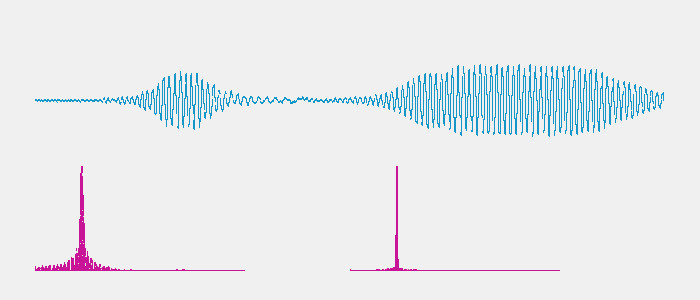
\includegraphics[scale=0.51]{./titre/heisenberg2}
\end{center}
%
\begin{itemize}[leftmargin=1cm, label=\ding{32}, itemsep=0pt]
\item Simulation numérique d'une corde vibrante.
\item Représentation graphique de la corde.
\item Calcul de la transformée de fourier.
\item Représentation du spectre.
\item Enregistrement et rechargement des situations.
\item Conditions initiales préenregistrées.
\end{itemize}
%
\subsection{SiCP, chaîne de pendules couplés}
%
\begin{center}
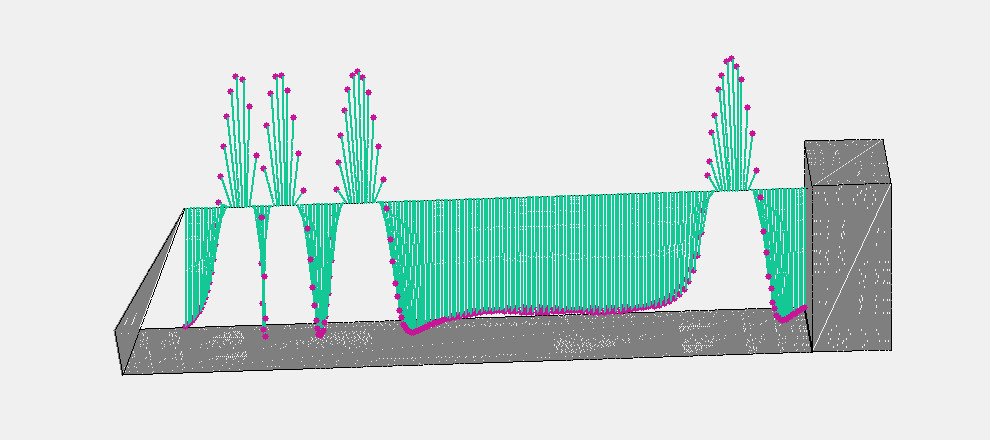
\includegraphics[scale=0.41]{./titre/SiCP}
\end{center}
%
\begin{itemize}[leftmargin=1cm, label=\ding{32}, itemsep=0pt]
\item Nombre de pendule variable.
\item Simulation de l'équation de sine-gordon et du courant josephson.
\item Graphisme en 3 dimensions, déplacement du point du vue.
\end{itemize}
%
\subsection{SiGP, thermodynamique statistique}
%
Le simulateur de gaz parfait SiGP permet de visualiser une interprétation statistique de la détente de Joule, du démon de Maxwell ainsi que du contact avec un ou deux thermostats.
%
\begin{center}
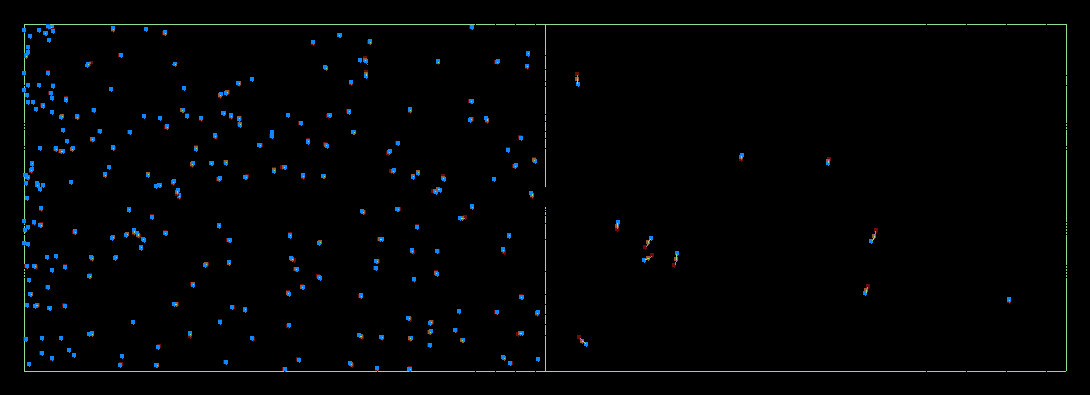
\includegraphics[scale=0.41]{./titre/SiGP}
\end{center}
%
\begin{itemize}[leftmargin=1cm, label=\ding{32}, itemsep=0pt]
\item Simulation de collisions élastiques.
\item Représentation graphique. 
\item Ajustement de la température des parois.
\item Paroi centrale et détente de joule.
\item Paroi centrale et démon de Maxwel.
\end{itemize}
%
%
\section{Installation des simulateurs}
Cette section traite de l'installation des simulateurs SiGP, SiCF et SiCP sur un système d'exploitation de type debian. Le téléchargement se fait avec un navigateur internet, la compilation et l'exécution se font dans un terminal. L'installation des outils de compilation nécessite les privilèges du super-utilisateur.
\begin{itemize}[leftmargin=1cm, label=\ding{32}, itemsep=0pt]
\item {\bf Installation des outils de compilation}
	\begin{itemize}[leftmargin=1cm, label=\ding{32}, itemsep=0pt]
	\item \texttt{sudo apt-get install gcc make libsdl-dev}
	\end{itemize}
\item {\bf Téléchargement des sources}
	\begin{itemize}[leftmargin=1cm, label=\ding{32}, itemsep=0pt]
	\item Télécharger les fichiers \texttt{.zip} sur github
		\begin{itemize}[leftmargin=1cm, label=\ding{32}, itemsep=0pt]
		\item \texttt{https://github.com/runigo/SiCP/archive/master.zip}
		\item \texttt{https://github.com/runigo/SiCF/archive/master.zip}
		\item \texttt{https://github.com/runigo/SiGP/archive/master.zip}
		\end{itemize}
	\item Décompresser les fichiers \texttt{.zip}
		\begin{itemize}[leftmargin=1cm, label=\ding{32}, itemsep=0pt]
		\item \texttt{unzip SiCP-master.zip}
		\item \texttt{unzip SiCF-master.zip}
		\item \texttt{unzip SiGP-master.zip}
		\end{itemize}
	\end{itemize}
\item {\bf Compilation}
	\begin{itemize}[leftmargin=1cm, label=\ding{32}, itemsep=0pt]
	\item La commande \texttt{make} dans le répertoire des sources produit un fichier exécutable :
		\begin{itemize}[leftmargin=1cm, label=\ding{32}, itemsep=0pt]
		\item \texttt{SiCF} pour SiCF
		\item \texttt{SiCP} pour SiCP
		\item \texttt{SiGP} pour SiGP
		\end{itemize}
	\end{itemize}

\item {\bf Exécution}
	\begin{itemize}[leftmargin=1cm, label=\ding{32}, itemsep=0pt]
	\item En ligne de commande, avec d'éventuelles options
		\begin{itemize}[leftmargin=1cm, label=\ding{32}, itemsep=0pt]
		\item \texttt{./SiCF [OPTION]}
		\item \texttt{./SiCP [OPTION]}
		\item \texttt{./SiGP [OPTION]}
		\end{itemize}
	\item La fenêtre graphique donne une représentation de la simulation,
	\item Le terminal affiche les informations.
	\end{itemize}
\end{itemize}





\newpage

%%%%%%%%%%%%%%%%%%%%%%%%%%%%%%%%%%%
\section{Commandes des simulateurs}
%%%%%%%%%%%%%%%%%%%%%%%%%%%%%%%%%%%

Cette section traite des interactions entre le programme et l'utilisateur.

\subsection{Commande du simulateur de gaz parfait SiGP}

Lorsque le programme est démarré en ligne de commande, il est possible de passer un certain nombre d'option. Elle sont communiqué au programme à l'aide du nom de l'option suivies d'un nombre. Par exemple pour démarrer SiGP avec un fond sombre, deux fluxons et une discrétisation du temps égale à 0,033 seconde :

\begin{center}
\texttt{./SiGP cf 17 df 2 dt 0.033}
\end{center}

\subsubsection{Options et commande du clavier}

\begin{center}
\begin{tabular}{cccc}
option & valeur & clavier & commande \\
\hline
pause & 5 < d < 555 &  & pause entre les affichages en ms \\
%duree & 1 < d < 99 & flèches & nombre d'évolution du système entre les affichages \\
duree & 1 < d < 99 & flèches & vitesse de la simulation \\
cloison & -3 < d < 3 & \texttt{w-n} & cloison si <> 0 \\
thermostat & -2 < d < 2 & \texttt{o} , \texttt{l} & système isolé si = 0 \\
vitesse & 0.03 < f < 33.3 &  & Vitesse initiale \\
temperature & 0.0000003 < f < 90 000 & \texttt{p}, \texttt{m} & Température thermostat \\
gauche & 0.0000003 < f < 90 000 & \texttt{u}, \texttt{j} & Thermostat gauche \\
droite & 0.0000003 < f < 90 000 & \texttt{i}, \texttt{k} & Thermostat droite \\
\end{tabular}
\end{center}

\subsubsection{Cloison centrale}

	{\it Option} : 

\begin{itemize}[leftmargin=1cm, label=\ding{32}, itemsep=0pt]
\item 0: {\bf Pas de cloison}
\item 1: {\bf Cloison percée.}
\item 2: {\bf Cloison}
\item -1: {\bf Cloison percée et démon de maxwell.}
\item -2: {\bf Cloison et démon de maxwell}
\end{itemize}

	{\it Clavier} : 

\begin{itemize}[leftmargin=1cm, label=\ding{32}, itemsep=0pt]
\item w: {\bf Pas de cloison}
\item x: {\bf Cloison percée}
\item c: {\bf Cloison}
\item b: {\bf Cloison percée et démon de maxwell.}
\item n: {\bf Cloison et démon de maxwell.}
\end{itemize}

\subsubsection{Thermostat}

	{\it Option} : 

\begin{itemize}[leftmargin=1cm, label=\ding{32}, itemsep=0pt]
\item 0: {\bf Système isolé}
\item 1: {\bf Température gauche-droite identiques}
\item 2: {\bf Température gauche-droite différentes}
\end{itemize}

	{\it Clavier} : 

\begin{itemize}[leftmargin=1cm, label=\ding{32}, itemsep=0pt]
\item o: {\bf Système isolé}
\item l: {\bf Température gauche-droite identiques}
\item l: {\bf Température gauche-droite différentes}
\end{itemize}

\texttt{mo} : {\bf Mode -1 : Wait, 1 : Poll} %optionsMode(option, opt[i+1]);
  (mode == 1 || mode == -1)

\normalsize


\subsection{Option de la ligne de commande de SiCP 1.3}
Lorsque le programme est démarré en ligne de commande, il est possible de passer un certain nombre d'option. Elle sont communiqué au programme à l'aide de deux lettres suivies d'un nombre. Par exemple pour démarrer SiCP avec un fond sombre, deux fluxons et une discrétisation du temps égale à 0,0033 seconde :
\begin{center}
\texttt{./SiCP fond 17 soliton 2 dt 0.0033}
\end{center}
Les options possibles sont :
\begin{itemize}[leftmargin=2cm, label=\ding{32}, itemsep=3pt]
\item {\large \texttt{nombre}} : {\bf Nombre de pendules.} %optionsDephasage(option, opt[i+1]);
  (nombre > 2 \&\& nombre < NOMBRE\_MAX). Initialise le nombre de pendules couplés.
\item {\large \texttt{soliton}} : {\bf déphasage entre les extrémitées.} %optionsDephasage(option, opt[i+1]);
  (soliton > -99 \&\& soliton < 99). Initialise le déphasage entre le dernier pendule et le premier pendule dans le cas des conditions aux limites périodique.
\item {\large \texttt{equation}} : {\bf choix de l'équation} %optionsEquation(option, opt[i+1]);
  (equation > 0 \&\& equation < 5).  Calcul de la FORCE DE RAPPEL (gamma est négatif)
\begin{itemize}[leftmargin=1cm, label=\ding{32}, itemsep=0pt]
\item 1: {\bf gravitation} forceRappel = sinus de la position du pendule
\item 2: {\bf linearisation} forceRappel = proportionnelle à la position du pendule
\item 3: {\bf corde vibrante} forceRappel = 0
\item 4: {\bf corde vibrante asymétrique} forceRappel = 0
\end{itemize}
%\item default:// corde vibrante forceRappel = 0.0;
\item {\large \texttt{fond}} : {\bf Couleur du fond} %optionsFond(option, opt[i+1]);
  (fond>0 \&\& fond<255)
%\item {\Large \texttt{th}} Deux threads %optionsThread(option, opt[i+1]);
  %(thread==1 || thread==0)
%\item {\large \texttt{mo}} : {\bf Mode -1 : Wait, 1 : Poll} %optionsMode(option, opt[i+1]);
%  (mode == 1 || mode == -1)
\item {\large \texttt{pause}} : {\bf temps de pause en ms} %optionsPause(option, opt[i+1]);
  (pause > 5 || pause < 555)
\item {\large \texttt{dt}} : {\bf discrétisation du temps} %optionsDt(option, opt[i+1]);
  (dt > 0.0 \&\& dt < DT\_MAX)
\end{itemize}

\subsection{Option de la ligne de commande de SiCP64 1.1}
Lorsque le programme est démarré en ligne de commande, il est possible de passer un certain nombre d'option. Elle sont communiqué au programme à l'aide du nom de l'option suivies d'un nombre. Par exemple pour démarrer SiCP64 avec un fond sombre, deux fluxons et une discrétisation du temps égale à 0,033 seconde :
\begin{center}
\texttt{./SiCP64 cf 17 df 2 dt 0.033}
\end{center}
Les options possibles sont :
\begin{itemize}[leftmargin=2cm, label=\ding{32}, itemsep=3pt]
\item {\large \texttt{df}} : {\bf déphasage entre les extrémitées.} %optionsDephasage(option, opt[i+1]);
  (fluxon > -99 \&\& fluxon < 99). Initialise le déphasage entre le dernier pendule et le premier pendule dans le cas des conditions aux limites périodique.
\item {\large \texttt{eq}} : {\bf choix de l'équation} %optionsEquation(option, opt[i+1]);
  (equation > 0 \&\& equation < 5).  Calcul de la FORCE DE RAPPEL (gamma est négatif)
\begin{itemize}[leftmargin=1cm, label=\ding{32}, itemsep=0pt]
\item 1: {\bf gravitation} forceRappel = sinus de la position du pendule
\item 2: {\bf linearisation} forceRappel = proportionnelle à la position du pendule
\item 3: {\bf corde vibrante} forceRappel = 0
\item 4: {\bf corde vibrante asymétrique} forceRappel = 0
\end{itemize}
%\item default:// corde vibrante forceRappel = 0.0;
\item {\large \texttt{cf}} : {\bf Couleur du fond} %optionsFond(option, opt[i+1]);
  (fond>0 \&\& fond<255)
%\item {\Large \texttt{th}} Deux threads %optionsThread(option, opt[i+1]);
  %(thread==1 || thread==0)
\item {\large \texttt{mo}} : {\bf Mode -1 : Wait, 1 : Poll} %optionsMode(option, opt[i+1]);
  (mode == 1 || mode == -1)
\item {\large \texttt{po}} : {\bf temps de pause en ms} %optionsPause(option, opt[i+1]);
  (pause > 5 || pause < 555)
\item {\large \texttt{dt}} : {\bf discrétisation du temps} %optionsDt(option, opt[i+1]);
  (dt > 0.0 \&\& dt < DT\_MAX)
\end{itemize}

\subsection{Commande du clavier}

\subsubsection{Résumé SiCP64 1.1}
\begin{center}
\begin{tabular}{cccccccccc}
%\sffamily
%\rmfamily
\sf A &\sf Z &\sf E &\sf R &\sf T &\sf Y &\sf U &\sf I &\sf O &\sf P \\
Couplage & Masse & Dissip. & supprimD & Gravit. & Phi & Sym. & impuls. & sinCar & fréquence \\
\sf Q &\sf S &\sf D &\sf F &\sf G &\sf H &\sf J &\sf K &\sf L &\sf M \\
moinsC & moinsM & plusD & formeD & moinsG & moins$\Phi$ & moinsS & Ampl. & moinsA & moinsF \\
\sf W &\sf X &\sf C &\sf V &\sf B &\sf N &  &  &  & \\
périodique & libres & fixe & ExtAbsD & libFix & fixLib &  &  &  & \\
\end{tabular}
\end{center}
\vspace{.3cm}
\begin{center}
\begin{tabular}{ccccc ccccc cc}
%\sffamily
%\rmfamily
\multicolumn{4}{|c|}{Contrôles} & \multicolumn{4}{c}{Information} & \multicolumn{4}{|c|}{SiCP64}\\
\sf F1 &\sf F2 &\sf F3 &\sf F4 &\sf F5 &\sf F6 &\sf F7 &\sf F8 &\sf F9 &\sf F10 &\sf F11 &\sf F12 \\
Mode & -Sim & +Sim &  & Énergie  &  &  &   & Altitude & gauche & droite & Altitude \\
\sf Entrée &\sf - &\sf + &\sf  &\sf  &\sf  &\sf  &\sf  &\sf  &\sf  \\
Mode & -Sim & +Sim & & & & & & & \\
\end{tabular}
\end{center}
\subsubsection{Résumé SiCP 1.3}
\begin{center}
\begin{tabular}{cccccccccc}
%\sffamily
%\rmfamily
\sf A &\sf Z &\sf E &\sf R &\sf T &\sf Y &\sf U &\sf I &\sf O &\sf P \\
Couplage & Masse & Dissip. & supprimD & Gravit. & Phi & Sym. & impuls. & sinCar & fréquence \\
\sf Q &\sf S &\sf D &\sf F &\sf G &\sf H &\sf J &\sf K &\sf L &\sf M \\
moinsC & moinsM & plusD & formeD & moinsG & moins$\Phi$ & moinsS & Ampl. & moinsA & moinsF \\
\sf W &\sf X &\sf C &\sf V &\sf B &\sf N &  &  &  & \\
périodique & libres & fixe & ExtAbsD & libFix & fixLib &  &  &  & \\
\end{tabular}
\end{center}
\vspace{.3cm}
\begin{center}
\begin{tabular}{ccccc ccccc cc}
%\sffamily
%\rmfamily
\multicolumn{4}{|c|}{Contrôles} & \multicolumn{4}{c}{Information} & \multicolumn{4}{|c|}{SiCP}\\
\sf F1 &\sf F2 &\sf F3 &\sf F4 &\sf F5 &\sf F6 &\sf F7 &\sf F8 &\sf F9 &\sf F10 &\sf F11 &\sf F12 \\
Pendules & Harmoniques & Corde & asymétrique & Énergie &  &  &   &  &  &  &  \\
\sf Entrée &\sf - &\sf + &\sf  &\sf  &\sf  &\sf  &\sf  &\sf  &\sf  \\
Mode & -Sim & +Sim & & & & & & & \\
\end{tabular}
\end{center}
%
\subsubsection{Paramètres de la chaîne}
%
\begin{itemize}[label=\ding{32}, leftmargin=2cm]
\item {\bf Couplage} : \texttt{a, q} : Augmente, diminue le couplage entre les pendules.
\item {\bf Masse} : \texttt{z, s} :  Augmente, diminue la masse des pendules.
\item {\bf Dissipation} : \texttt{e, d} :  Augmente, diminue les frottements visqueux.
\item {\bf Gravitation} : \texttt{t, g} :  Augmente, diminue l'accélération de la gravitation.
%\item {\bf } : \texttt{} : 
\end{itemize}
%
\subsubsection{Forme de la dissipation}
%
\begin{itemize}[label=\ding{32}, leftmargin=2cm]
\item {\bf Supprimer} : \texttt{e} : Supprime les frottements visqueux.
\item {\bf Former} : \texttt{f} : Active les frottements visqueux sur toute la chaîne.
\item {\bf Absorber} : \texttt{v} : Active les frottements visqueux sur la fin de la chaîne, crée une extrémité absorbante.
\end{itemize}
%
\subsubsection{Conditions aux limites}
%
\begin{itemize}[label=\ding{32}, leftmargin=2cm]
\item {\bf Périodique} : \texttt{w} : Le dernier pendule est couplé au premier.
\item {\bf Libres} : \texttt{x} : Les deux extrémités sont libres.
\item {\bf Fixes} : \texttt{c} : Les deux extrémités sont fixes.
\item {\bf libre-fixe} : \texttt{b} : Le premier pendule est libre et le dernier pendule est fixe.
\item {\bf fixe-libre} : \texttt{n} : Le premier pendule est fixe et le dernier pendule est libre.
\end{itemize}
%
\subsubsection{Moteur premier pendule}
%
\begin{itemize}[label=\ding{32}, leftmargin=2cm]
\item {\bf Impulsion} : \texttt{i} : Crée une impulsion.
\item {\bf Sinus} : \texttt{o} : Active, désactive le moteur sinusoïdale.
\item {\bf Amplitude} : \texttt{k, l} :  Augmente, diminue l'amplitude du moteur.
\item {\bf Fréquence} : \texttt{p, m} :  Augmente, diminue la fréquence du moteur.
\end{itemize}
%
\subsubsection{Moteur Josephson}
%
\begin{itemize}[label=\ding{32}, leftmargin=2cm]
\item {\bf Activation} : \texttt{$\rightarrow$} : Crée, supprime un courant josephson.
\item {\bf Amplitude} : \texttt{$\uparrow, \downarrow$} : Augmente, diminue le courant.
\item {\bf Sens} : \texttt{$\leftarrow$} : Inverse le sens du courant josephson.
%\item {\bf } : \texttt{} : 
\end{itemize}
%
\subsubsection{Contrôle de la simulation}
%
\begin{itemize}[label=\ding{32}, leftmargin=2cm]
\item {\bf Mode} : \texttt{Entrée} ou \texttt{F1} : Change le mode de la simulation : temps réèl ou pas à pas.
\item {\bf Accélèrer} : \texttt{+} ou \texttt{F2} : Accélère la simulation.
\item {\bf Ralentir} : \texttt{-} ou \texttt{F3} : Ralentit la simulation.
%\item {\bf } : \texttt{} : 
\end{itemize}
%
\subsubsection{Information}
\begin{itemize}[label=\ding{32}, leftmargin=2cm]
\item {\bf Énergie} : \texttt{F5} : Information énergetique de la chaîne.
%\item {\bf } : \texttt{F6} : 
%\item {\bf } : \texttt{F7} : 
%\item {\bf } : \texttt{F8} : 
\end{itemize}
%
\subsubsection{Graphisme SiCP64}
%
\begin{itemize}[label=\ding{32}, leftmargin=2cm]
\item {\bf Altitude} : \texttt{F9} : Diminue l'altitude du point de vue.
\item {\bf Rotation} : \texttt{F10} : Tourne la chaîne vers la gauche.
\item {\bf Rotation} : \texttt{F11} : Tourne la chaîne vers la droite.
\item {\bf Altitude} : \texttt{F12} : Augmente l'altitude du point de vue.
\end{itemize}
%
\subsection{Commande de la souris}
%
\subsubsection{Graphisme SiCP64}
%
Cliquer et déplacer le pointeur de la souris permet de déplacer le point de vue de l'observateur.
\subsection{Enregistrement de la position}

\subsubsection{Dans SiCP64}
%
La touche majuscule permet d'accéder aux fonctions d'enregistrement et de réinitialisation des positions des pendules.
%\item {\bf } : \texttt{} : 
%%%%%%%%%%%%%%%%%%%%%%%%%%%%%%%%%%%%%%%%%%%%%%%%%%%%%%%%%ù

%
%
%%%%%%%%%%%%%%%%%%%%%%
\section{Exemples}
%%%%%%%%%%%%%%%%%%%%%%

Cette section traite de la mise en marche et des premières utilisation de SiCF

\subsection{Dissipation}
\begin{itemize}[label=\ding{32}, leftmargin=2cm]
\item \texttt{texte} : texte
\end{itemize}
%
\subsection{Conditions aux limites}
\begin{itemize}[label=\ding{32}, leftmargin=2cm]
\item Périodique
\item libre
\item fixe
\end{itemize}
%
\subsection{Transformée de fourier}
%
\subsection{Réalisation d'un paquet d'onde}
%
\subsection{Inégalité de Heisenberg}
%
\subsection{}



%%%%%%%%%%%%%%%%%%%%%%%%%%%%%%%%%%%%%%%%%%%%%%%%%%%%%%%%%%%%%%%%%%%%%%


%
\chapter{Modèles physiques}
%
Ce chapitre traite des modèles physiques liés aux phénomènes abordés par les simulateurs.
%
%%%%%%%%%%%%%%%%%%%%%%%%%%%%%%
\section{La chaine de pendule}
%%%%%%%%%%%%%%%%%%%%%%%%%%%%%%
\subsection{La chaine de pendule}
\label{chaineDePendule}
\subsubsection{L'équation de la chaine de pendule}
La chaîne de pendule est constituée d'une série de pendules pesants. Chaque pendule étant couplé avec ses deux plus proches voisins à l'aide d'un fil de torsion.\cite{sine-gordon}\cite{chaine-pendule}
\[
\frac{\mathrm d^2\theta _n}{\mathrm d t^2} - c^2 \frac{\theta _{n+1} + \theta _{n-1} - 2 \theta _n}{\mathrm{a} ^2} + \omega _0 ^2 \sin \theta _n = 0
\]
%
\begin{center}
\begin{tabular}{cccc}
%\multicolumn{4}{|c|}{Contrôles} & \multicolumn{4}{c}{Information} & \multicolumn{4}{|c|}{Contrôles}\\
$\frac{k}{m}$ & $\frac{vitesse^2}{longueur^2}$ & T$^{-2}$ & $\frac{k}{m}$ = $\frac{c^2}{a^2}$ \\
$\frac{g}{l}$& pulsation$^2$ & T$^{-2}$ & $\frac{g}{l}$ = $\omega _0 ^2$ \\
\end{tabular}
\end{center}
%

La relation fondamentale de la dynamique, donne, en prennant en compte les frottements visqueux :
%
\[
m l\ \frac{d^2 \theta _n}{\dt^2} =  - m g \sin{\theta _n}  -  k l \Delta \theta _n(t)  -  \beta\ \frac{d \theta _n}{\dt}
\]
%
\begin{center}
\begin{tabular}{cccccc}
%\multicolumn{4}{|c|}{Contrôles} & \multicolumn{4}{c}{Information} & \multicolumn{4}{|c|}{Contrôles}\\
avec & & $\theta _n$ & angle & radian &  \\
 & & m & masse & M &  \\
 & & g & pesanteur & LT$^{-2}$ &  \\
 & & k & torsion & MT$^{-2}$ &  \\
 & & l & longueur & L &  \\
 & & $\beta$ & frottement & ML$^{2}$T$^{-1}$ &  \\
\end{tabular}
\end{center}
%
\subsubsection{Expressions de l'énergie}

La force de rappel, s'exerçant sur la masse m, dû au fil de torsion entre les pendules est :
\[
f_{torsion} = -  k l \Delta \theta _n = -  k l\ (2\theta _n-\theta _{n-1}-\theta _{n+1})
\]

L'énergie potentielle entre les pendules n et n-1 est :
\[
E_{couplage} = \frac{1}{2}\ k l^2 (\theta _n-\theta _{n-1})^2
\]

La force de rappel dû à la gravitation est :
\[
f_{gravitation} = - m g \sin{\theta _n}
\]

L'énergie potentielle de pesanteur de la masse m est :
\[
E_{pp} = m g l (1 - \cos{\theta _n})
\]

La linéarisation de cette dernière force aboutit à une force de rappel harmonique :
\[
f_{ressort} = - m g \theta _n
\]

L'énergie potentielle correspondante est alors:
\[
E_{pp} = \frac{1}{2}\ m g l \theta _n^2
\]

Enfin, l'énergie cinétique découle du travail de 
\[
m l\ \frac{d^2 \theta _n}{\dt^2}
\]
%
Et vaut
\[
E_{c} = \frac{1}{2}\ m l (\frac{d \theta _n}{\dt})^2
\]


La force de frottement visqueux est :
%
\[
f_{frottement} = -  \beta\ \frac{\theta _n(t) - \theta _n(t-\dt)}{\dt}
\]
%
La présence de cette force implique une dissipation de l'énergie. En l'absence de cette force, on doit observer une conservation de l'énergie totale.

À ces forces il faut ajouter le courant josephson, correspondant à une constante additive dans la relation fondamentale de la dynamique ainsi que la force s'xerçant sur le premier pendule lors de l'excitation de la chaîne.
%%%%%%%%%%%%%%%%%%%%%%%%%%%%%%%%%%%%%%%%%%%%%%%%%%%%%%%%%%%%%%%%%
%La relation fondamentale de la dynamique donne :
%\[- m g \sin{\theta _n(t)}  -  k l \Delta \theta _n(t)  -  \beta\ \frac{\theta _n(t) - \theta _n(t-\dt)}{\dt} =  m l\ \frac{\theta _n(t+\dt) - 2\theta _n(t) + \theta _n(t-\dt)}{\dt^2}\]
%soit\[\frac{\theta _n(t+\dt) - 2\theta _n(t) + \theta _n(t-\dt)}{\dt^2} = - \frac{g}{l} \sin{\theta _n(t)}  -  \frac{k}{m} \Delta \theta _n(t)  -  \frac{\beta}{ml}\ \frac{\theta _n(t) - \theta _n(t-\dt)}{\dt}\]
%D'ou finallement\[\theta _n(t+\dt) = 2\theta _n(t) - \theta _n(t-\dt) + \delta force_n\]
%avec \[\delta force_n = - \dt^2 \frac{g}{l} \sin{\theta _n(t)} - \dt^2 \frac{k}{m} \Delta \theta _n(t) - \dt \frac{\beta}{ml} (\theta _n(t) - \theta _n(t-\dt))\]
%%%%%%%%%%%%%%%%%%%%%%%%%%%%%%%%%%%%%%%%%%%%%%%%%%%%%%%%%%%%%%%%%

%
%%%%%%%%%%%%%%%%%%%%%
\section{L'équation de Sine-Gordon}
%%%%%%%%%%%%%%%%%%%%%
%
Cette section traite de l'équation de sine-gordon et de ses solutions
\subsection{L'équation de Sine-Gordon}
C'est une équation différentielle du second ordre, non linéaire, à deux variables \cite{sine-gordon}.
\[
\frac{\partial^2\theta}{\partial t^2} - c^2 \frac{\partial^2\theta}{\partial x^2} + \omega _0 ^2 \sin \theta = 0
\]
%
%
%
\subsection{Les solitons, solutions de l'équation de Sine-Gordon}
Une solution de l'équation de Sine-Gordon, appelée soliton, est 
\[
\theta(x,t)=4\arctan \exp ( \omega t - \text{k} x )
\]
%\[ \mbox{Let } x = \mbox{ number of cats} \]%\text{$$}
%\[ \textrm{Let } x = \textrm{ number of cats} \]
Elle correspond à une variation de 2$\pi$ de la valeur de $\theta$ sur une distance de l'ordre de k$^{-1}$. Le soliton se déplace à la vitesse v.
%c=$\omega / k $
\subsection{Phénomènes physiques associés aux solitons}
La {\bf jonction josephson}. Constitué par une jonction isolante entre deux supraconducteur.

Les {\bf motifs du pelage des animaux} \cite{pelage-animaux}

Les {\bf frontières}. New-York possède un quartier chinois et un quartier italien. Le grignotage de Little Italy par Chinatown montre le déplacement de la brutale variation des densités de population chinoise et italienne.

%%%%%%%%%%%%%%%%%%%%%%%%%%%%%%%%%%%%%%%%%%%%%%%%%%%%%%%%%%%%%%%%%%%%%%%%%%%%%%%%%%%%%

%
%%%%%%%%%%%%%%%%%%%%%
\section{La corde vibrante}
%%%%%%%%%%%%%%%%%%%%%
%
Cette section traite de l'équation des cordes vibrantes, de ses solutions et de la transformée de fourier.
\subsection{La corde vibrante}
C'est une équation différentielle du second ordre, linéaire, à deux variables \cite{corde-vibrante}.
\[
\frac{\partial^2 u}{\partial t^2} - c^2 \frac{\partial^2 u}{\partial x^2} = 0
\]
%
%
%
\subsection{La transformée de fourrier}
%
La transformée de fourier correspond à la décomposition d'une fonction sur une base de fonctions harmoniques.
\[
\hat{u}(k) = \int_{-\infty}^{+\infty} u(x) \mathrm e^{-2 i \pi k x} \, \mathrm dx
\]
%
%
%
%%%%%%%%%%%%%%%%%%%%%%%%%%%%%%%%%%%%%%%%%%%%
%%%%%%%%%%%%%%%%%%%%%%%%%%%%%%%%%%%%%%%%%%%%%%%%%%%%%%%%%%%%%%%%%%%%%%%%%%%%%%%%%%%%%

%
%%%%%%%%%%%%%%%%%%%%%%%%%%%%%%%%%
\section{Les chocs de particules}
%%%%%%%%%%%%%%%%%%%%%%%%%%%%%%%%%
%
\subsection{Les chocs de particules}
On applique les lois de conservations de l'énergie et de l'impulsion :
\[
\sum m_i{v'_i}^2=\sum m_iv_i^2
\hspace{2cm}
\sum m_i\overrightarrow{v'}_i=\sum m_i\overrightarrow{v}_i
\]
\begin{center}
$\sum m_i{v'_i}^2=\sum m_iv_i^2$
\hspace{2cm}
$\sum m_i\overrightarrow{v'}_i=\sum m_i\overrightarrow{v}_i$
\end{center}
\begin{center}
$m_i\mathbf{v'}_i^2=m_i\mathbf{v}_i^2$
\hspace{2cm}
$m_i\mathbf{v'}_i=m_i\mathbf{v}_i$
\end{center}
%
\subsection{Chocs de deux particules}
La conservations de l'énergie donne :
\[
m_1{v'_1}^2 + m_2{v'_2}^2=m_1v_1^2 + m_2v_2^2
\]
La conservations de l'impulsion donne :
\[
m_1\overrightarrow{v'}_1 + m_2\overrightarrow{v'}_2=m_1\overrightarrow{v}_1 + m_2\overrightarrow{v}_2
\]
Dans le référentiel du centre de masse : 
\[
(m_1 + m_2)\overrightarrow{v}=m_1\overrightarrow{v}_1 + m_2\overrightarrow{v}_2
\]
%
%%%%%%%%%%%%%%%%%%%%%%%%%%%%%%%%%%%%%%%%%%%%
%%%%%%%%%%%%%%%%%%%%%%%%%%%%%%%%%%%%%%%%%%%%
%%%%%%%%%%%%%%%%%%%%%%%%%%%%%%%%%%%%%%%%%%%%%%%%%%%%%%%%%%%%%%%%%%%%%%%%%%%%%%%%%%%%%

%\chapter{Modèles physiques}
%
Ce chapitre traite des modèles physiques liés aux phénomènes abordés par les simulateurs.
%
%%%%%%%%%%%%%%%%%%%%%%%%%%%%%%
\section{La chaîne de pendule}
%%%%%%%%%%%%%%%%%%%%%%%%%%%%%%

\subsection{Le pendule pesant}
\begin{multicols}{2}%\columnbreak\end{multicols}
\begin{tikzpicture}
%\draw [ball color=gray] (0,0)coordinate(A)node[left]{$m$\ \ \ } circle (.3);
\draw [ball color=gray] (0,0)coordinate(A)node[below=3mm]{$m$} circle (.3);
\draw (0.21,0.21) -- (45:4.7)coordinate(B)node[right]{O}node[pos=.5,left=2mm]{$l$};
%\draw (0,0)coordinate(A)node[left]{m}circle(.1)-- (40:5)coordinate(B)node[right]{O};=3mm
\draw[dashed](B)--++(0,-5)coordinate(C);
\draw pic[ draw ,<->,"$\theta$",angle eccentricity =1.5, angle radius=1cm]{ angle =A--B--C};
%\draw[dotted,thick](0,0)arc(-135:-90:5);node[right]{B}
\draw [->](5,2) --++(0,-2)node[pos=.5,left]{$\overrightarrow{g}$};
\end{tikzpicture}

\columnbreak
Un pendule pesant est constitué par une masse $m$ suspendue à un fil rigide de longueur $l$ relié à un point O. Une liaison en ce point permet au pendule de tourner autour d'un axe fixe. L'angle entre le fil et la verticale est noté $\theta$. La masse est soumise à son poids $\overrightarrow{P}=m\overrightarrow{g}$, à la réaction du fil $\overrightarrow{R}$ et à une force de frottement visqueux $\overrightarrow{f}= - \frac{\beta}{l} \overrightarrow{v}$. La relation fondamentale de la dynamique donne :
\[
m l\ \frac{d^2 \theta}{\dt^2} =  - m g \sin{\theta}  -  \beta\ \frac{d \theta}{\dt}
\]
\end{multicols}
%
\subsection{Les pendules couplés}
\begin{multicols}{2}%\columnbreak\end{multicols}
Deux pendules pesants sont reliés par un fil de torsion suivant leur axe fixe commun.  La relation fondamentale de la dynamique donne alors :
\[\left\{
  \begin{array}{rcr}
m l\ \frac{d^2 \theta _1}{\dt^2} & = &  - m g \sin{\theta _1}  -  \beta\ \frac{d \theta _1}{\dt} - kl (\theta _1 - \theta _2) \\
m l\ \frac{d^2 \theta _2}{\dt^2} & = &  - m g \sin{\theta _2}  -  \beta\ \frac{d \theta _2}{\dt} - kl (\theta _2 - \theta _1) \\
  \end{array}
\right.\]
dans le cas où les pendules sont identiques.

\columnbreak
\begin{tikzpicture}
\draw [ball color=gray] (0,0)coordinate(A)node[below=3mm]{$m$} circle (.2);
\draw (0.13,0.13) -- (65:2.7)coordinate(B);%node[right]{O}node[pos=.5,left=2mm]{$l$};
\draw[dashed](B)--++(0,-3)coordinate(C);
\draw pic[ draw ,<->,"$\theta _1$",angle eccentricity =1.5, angle radius=1cm]{ angle =A--B--C};
%
\draw [ball color=gray] (3,0.3)coordinate(D)node[below=3mm]{$m$} circle (.2);
\draw (3.13,0.43) -- (35:5.1)coordinate(E);%node[right]{O}node[pos=.5,left=2mm]{$l$};
\draw[dashed](E)--++(0,-3)coordinate(F);
\draw pic[ draw ,<->,"$\theta _2$",angle eccentricity =1.5, angle radius=1cm]{ angle =D--E--F};
%
\draw[decorate,decoration={coil,segment length=10pt,amplitude=0.2cm,aspect=.8}](B)--(E)node[pos=.5,above=2mm]{$k$};
\end{tikzpicture}
\end{multicols}
%
%
%
\subsection{La chaîne de pendule}
Une chaîne de pendule est constituée d'une série de pendules pesants. Chaque pendule étant couplé avec ses deux plus proches voisins à l'aide d'un fil de torsion.

\begin{tikzpicture}[rotate=-10]
\foreach \x/\t/\a in {1/{}/0, 2/{}/2, 3/{}/5, 4/{\theta _{n-1}}/9, 5/{\theta _n}/14, 6/{\theta _{n+1}}/9, 7/{}/5, 8/{}/2, 9/{}/0}
{
\coordinate (A) at (1.5*\x,0) ;
\draw[decorate,decoration={coil,amplitude=0.07cm,aspect=1.1}](A)-- ++(1.5,0)coordinate(B);
\draw (B) -- ++(-90-\a:3)[ball color=gray] ++(0,0) circle (.2) node[below=2mm]{$\t$};
%\draw;
}
\end{tikzpicture}

\label{chaineDePendule}
\subsection{L'équation de la chaine de pendule}
La chaîne de pendule est constituée d'une série de pendules pesants. Chaque pendule étant couplé avec ses deux plus proches voisins à l'aide d'un fil de torsion.\cite{sine-gordon}\cite{chaine-pendule}
\[
\frac{\mathrm d^2\theta _n}{\mathrm d t^2} - c^2 \frac{\theta _{n+1} + \theta _{n-1} - 2 \theta _n}{\mathrm{a} ^2} + \omega _0 ^2 \sin \theta _n = 0
\]
%
\begin{center}
\begin{tabular}{cccc}
%\multicolumn{4}{|c|}{Contrôles} & \multicolumn{4}{c}{Information} & \multicolumn{4}{|c|}{Contrôles}\\
$\frac{k}{m}$ & $\frac{vitesse^2}{longueur^2}$ & T$^{-2}$ & $\frac{k}{m}$ = $\frac{c^2}{a^2}$ \\
$\frac{g}{l}$& pulsation$^2$ & T$^{-2}$ & $\frac{g}{l}$ = $\omega _0 ^2$ \\
\end{tabular}
\end{center}

La relation fondamentale de la dynamique, donne, en prennant en compte les frottements visqueux :
\[
m l\ \frac{d^2 \theta _n}{\dt^2} =  - m g \sin{\theta _n}  -  k l \Delta \theta _n(t)  -  \beta\ \frac{d \theta _n}{\dt}
\]
soit
\[
\frac{d^2 \theta _n}{\dt^2} =  - \frac{g}{l} \sin{\theta _n}  -  \frac{k}{m} \Delta \theta _n(t)  - \frac{\beta}{ml}\ \frac{d \theta _n}{\dt}
\]
avec
\begin{center}
\begin{tabular}{cccccc}
 & {\it abréviation} & {\it grandeur} & {\it unité} &  \\
 & $\theta _n$ & angle & radian &  \\
 & m & masse & M &  \\
 & g & pesanteur & LT$^{-2}$ &  \\
 & k & torsion & MT$^{-2}$ &  \\
 & l & longueur & L &  \\
 & $\beta$ & frottement & ML$^{2}$T$^{-1}$ &  \\
\end{tabular}
\end{center}
%
\subsection{Expressions des forces et des énergies associées}

La force de rappel, s'exerçant sur la masse m, dû au fil de torsion entre les pendules est :
\[
f_{torsion} = -  k l \Delta \theta _n = -  k l\ (2\theta _n-\theta _{n-1}-\theta _{n+1})
\]
L'énergie potentielle entre les pendules n et n-1 est :
\[
E_{couplage} = \frac{1}{2}\ k l^2 (\theta _n-\theta _{n-1})^2
\]

La force de rappel dû à la gravitation est :
\[
f_{gravitation} = - m g \sin{\theta _n}
\]
L'énergie potentielle de pesanteur de la masse m est :
\[
E_{pp} = m g l (1 - \cos{\theta _n})
\]
La linéarisation de cette dernière force donne lieu à une force de rappel harmonique :
\[
f_{ressort} = - m g \theta _n
\]
L'énergie potentielle correspondante est alors:
\[
E_{pp} = \frac{1}{2}\ m g l \theta _n^2
\]

Enfin, l'énergie cinétique découle du travail de 
\[
m l\ \frac{d^2 \theta _n}{\dt^2}
\]
%
Et vaut
\[
E_{c} = \frac{1}{2}\ m l (\frac{d \theta _n}{\dt})^2
\]


La force de frottement visqueux est :
%
\[
f_{frottement} = -  \beta\ \frac{\theta _n(t) - \theta _n(t-\dt)}{\dt}
\]
%
La présence de cette force implique une dissipation de l'énergie. En l'absence de cette force, on doit observer une conservation de l'énergie totale.

À ces forces il faut ajouter le courant josephson, correspondant à une constante additive dans la relation fondamentale de la dynamique ainsi que la force s'exerçant sur le premier pendule lors de l'excitation de la chaîne.
%%%%%%%%%%%%%%%%%%%%%%%%%%%%%%%%%%%%%%%%%%%%%%%%%%%%%%%%%%%%%%%%%
%La relation fondamentale de la dynamique donne :
%\[- m g \sin{\theta _n(t)}  -  k l \Delta \theta _n(t)  -  \beta\ \frac{\theta _n(t) - \theta _n(t-\dt)}{\dt} =  m l\ \frac{\theta _n(t+\dt) - 2\theta _n(t) + \theta _n(t-\dt)}{\dt^2}\]
%soit\[\frac{\theta _n(t+\dt) - 2\theta _n(t) + \theta _n(t-\dt)}{\dt^2} = - \frac{g}{l} \sin{\theta _n(t)}  -  \frac{k}{m} \Delta \theta _n(t)  -  \frac{\beta}{ml}\ \frac{\theta _n(t) - \theta _n(t-\dt)}{\dt}\]
%D'ou finallement\[\theta _n(t+\dt) = 2\theta _n(t) - \theta _n(t-\dt) + \delta force_n\]
%avec \[\delta force_n = - \dt^2 \frac{g}{l} \sin{\theta _n(t)} - \dt^2 \frac{k}{m} \Delta \theta _n(t) - \dt \frac{\beta}{ml} (\theta _n(t) - \theta _n(t-\dt))\]
%%%%%%%%%%%%%%%%%%%%%%%%%%%%%%%%%%%%%%%%%%%%%%%%%%%%%%%%%%%%%%%%%
\subsection{Résumé des forces et des énergies}
\begin{center}
\begin{tabular}{ccc}
%\multicolumn{4}{|c|}{Contrôles} & \multicolumn{4}{c}{Information} & \multicolumn{4}{|c|}{Contrôles}\\
 & force & énergie \\
torsion & -  k l $\Delta \theta _n$ & $\frac{1}{2}$ k l$^2 (\theta _n-\theta _{n-1})^2$ \\
gravitation & - m g $\sin{\theta _n}$ & m g l (1 - $\cos{\theta _n}$) \\
harmonique & - m g $\theta _n$ & $\frac{1}{2}$ m g l $\theta _n^2$ \\
inertie & m l $\frac{d^2 \theta _n}{\dt^2}$ & $\frac{1}{2}$ m l$^2$ $(\frac{d \theta _n}{\dt})^2$ \\
courant & josephson & \\
\end{tabular}
\end{center}
%

%
%%%%%%%%%%%%%%%%%%%%%
\section{L'équation de Sine-Gordon}
%%%%%%%%%%%%%%%%%%%%%
%
Cette section traite de l'équation de sine-gordon et de ses solutions
\subsection{L'équation de Sine-Gordon}
\label{belmont}
C'est une équation différentielle du second ordre, non linéaire, à deux variables \cite{sine-gordon}.
\[
\frac{\partial^2\theta}{\partial t^2} - c^2 \frac{\partial^2\theta}{\partial x^2} + \omega _0 ^2 \sin \theta = 0
\]
%
%
%
\subsection{Les solitons, solutions de l'équation de Sine-Gordon}
Une solution de l'équation de Sine-Gordon, appelée soliton, est 
\[
\theta(x,t)=4\arctan \exp ( \omega t - \text{k} x )
\]
%\[ \mbox{Let } x = \mbox{ number of cats} \]%\text{$$}
%\[ \textrm{Let } x = \textrm{ number of cats} \]
Elle correspond à une variation de 2$\pi$ de la valeur de $\theta$ sur une distance de l'ordre de k$^{-1}$. Le soliton se déplace à la vitesse v.
%c=$\omega / k $
\subsection{Phénomènes physiques associés aux solitons}
La {\bf jonction josephson}. Constitué par une jonction isolante entre deux supraconducteur.

%%%%%%%%%%%%%%%%%%%%%%%%%%%%%%%%%%%%%%%%%%%%%%%%%%%%%%%%%%%%%%%%%%%%%%%%%%%%%%%%%%%%%

%
%%%%%%%%%%%%%%%%%%%%%
\section{La corde vibrante}
%%%%%%%%%%%%%%%%%%%%%
%
Cette section traite de l'équation des cordes vibrantes, de ses solutions et de la transformée de fourier.
\subsection{La corde vibrante}
\label{boutin}
C'est une équation différentielle du second ordre, linéaire, à deux variables \cite{corde-vibrante}.
\[
\frac{\partial^2 u}{\partial t^2} - c^2 \frac{\partial^2 u}{\partial x^2} = 0
\]
%
%
%
\subsection{La transformée de fourrier}
\label{rodier}
%
La transformée de fourier correspond à la décomposition d'une fonction sur une base de fonctions harmoniques. \cite{fourier}
\[
\hat{u}(k) = \int_{-\infty}^{+\infty} u(x) \mathrm e^{-2 i \pi k x} \, \mathrm dx
\]
%
%
%
%%%%%%%%%%%%%%%%%%%%%%%%%%%%%%%%%%%%%%%%%%%%
%%%%%%%%%%%%%%%%%%%%%%%%%%%%%%%%%%%%%%%%%%%%%%%%%%%%%%%%%%%%%%%%%%%%%%%%%%%%%%%%%%%%%

%
%%%%%%%%%%%%%%%%%%%%%%%%%%%%%%%%%
\section{Les chocs de particules}
%%%%%%%%%%%%%%%%%%%%%%%%%%%%%%%%%
%
\subsection{Les chocs de particules}
On applique les lois de conservations de l'énergie et de l'impulsion :
%\[
%\sum m_i{v'_i}^2=\sum m_iv_i^2
%\hspace{2cm}
%\sum m_i\overrightarrow{v'}_i=\sum m_i\overrightarrow{v}_i
%\]
\begin{center}
$\sum m_i{v'_i}^2=\sum m_iv_i^2$
\hspace{2cm} et \hspace{2cm}
$\sum m_i\overrightarrow{v'}_i=\sum m_i\overrightarrow{v}_i$
\end{center}
ou en utilisant la convention de sommation sur les indices répétés :
\begin{center}
$m_i\mathbf{v'}_i^2=m_i\mathbf{v}_i^2$
\hspace{2cm} et \hspace{2cm}
$m_i\mathbf{v'}_i=m_i\mathbf{v}_i$
\end{center}
%
\subsection{Chocs de deux particules}
La conservation de l'énergie donne :
\[
m_1{v'_1}^2 + m_2{v'_2}^2=m_1v_1^2 + m_2v_2^2
\]
La conservation de l'impulsion donne :
\[
m_1\overrightarrow{v'}_1 + m_2\overrightarrow{v'}_2=m_1\overrightarrow{v}_1 + m_2\overrightarrow{v}_2
\]
Dans le référentiel du centre de masse : 
\[
(m_1 + m_2)\overrightarrow{v}=m_1\overrightarrow{v}_1 + m_2\overrightarrow{v}_2
\]
%
%%%%%%%%%%%%%%%%%%%%%%%%%%%%%%%%%%%%%%%%%%%%
%%%%%%%%%%%%%%%%%%%%%%%%%%%%%%%%%%%%%%%%%%%%
%%%%%%%%%%%%%%%%%%%%%%%%%%%%%%%%%%%%%%%%%%%%%%%%%%%%%%%%%%%%%%%%%%%%%%%%%%%%%%%%%%%%%

%\chapter{Modèles physiques}
%
Ce chapitre traite des modèles physiques liés aux phénomènes abordés par les simulateurs.
%
\input{./physique/chaine-pendule.tex}
\input{./physique/sine-gordon.tex}
\input{./physique/corde-vibrante.tex}
\input{./physique/choc-particule.tex}
%\input{./physique/physique.tex}
%
%%%%%%%%%%%%%%%%%%%%%%%%%%%%%%%%%%%%%%%%%%%%%%%%%%%%%%%%%%%%%%%%%%%%%%%%%%%%%%%%%%%%

%
%%%%%%%%%%%%%%%%%%%%%%%%%%%%%%%%%%%%%%%%%%%%%%%%%%%%%%%%%%%%%%%%%%%%%%%%%%%%%%%%%%%%

%
%%%%%%%%%%%%%%%%%%%%%%%%%%%%%%%%%%%%%%%%%%%%%%%%%%%%%%%%%%%%%%%%%%%%%%%%%%%%%%%%%%%%

%
\chapter{Mathématique et numérique}
%
Ce chapitre traite des modèles mathématiques et numériques liés aux simulateurs.
%

%%%%%%%%%%%%%%%%%%%%%
\section{Discrétisation}
%%%%%%%%%%%%%%%%%%%%%
%
La discrétisation de l'équation du mouvement se fait à l'aide de l'algorithme de Verlet. Cet algorithme consiste à symétriser la dérivée par rapport au temps puis d'obtenir une expression de $x(t+\dt)$ en fonction de $x(t)$ et $x(t-\dt)$. Cette expression permet de simuler de proche en proche le comportement du système physique. La solution discrète se rapproche de la solution analytique si la valeur de dt est convenablement choisie. En dehors d'un certain encadrement de dt, la solution discrète s'éloigne de la solution analytique.
%
\subsection{Discrétisation des dérivées}
%
\subsubsection{Dérivé symétrisée}
Par définition, la dérivé symétrique est :
\[
\frac{dx}{\dt}=\frac{x(t+\dt)-x(t-\dt)}{2\dt}
\]
On en déduit l'expression suivante de la dérivée seconde :
\[
\frac{d^2x}{\dt^2}=\frac{x(t+2\dt)-x(t)-x(t)+x(t-2\dt)}{4\dt^2}
\]
Le changement de variable dt' = 2 dt simplifie cette expression :
\[
\frac{d^2x}{\dt^2}=\frac{x(t+\dt)-2x(t)+x(t-\dt)}{\dt^2}
\]
Une expression disymétrique de la vitesse peut être utilisée pour l'évaluation des forces de viscosité ainsi que pour le calcul de l'énergie cinétique avant le calcul de la nouvelle valeur de $x(t+\dt)$.
\[
\frac{dx}{\dt}=\frac{x(t+\dt)-x(t)}{\dt}
\]
{\footnotesize Après l'incrémentation, } $\frac{dx}{\dt}=\frac{x(t)-x(t-\dt)}{\dt}$
%
\subsection{Discrétisation de la relation fondamentale de la dynamique}
%
L'équation de la chaîne de pendules couplés (\ref{chaineDePendule}) donne ici :
%
\[
\frac{x(t+\dt) - 2x(t) + x(t-\dt)}{\dt^2} = - \frac{g}{l} \sin{x(t)}  -  \frac{k}{m} \Delta x(t)  -  \frac{\beta}{ml}\ \frac{x(t) - x(t-\dt)}{\dt}
\]
soit
\[
x(t+\dt) - 2x(t) + x(t-\dt) = - \frac{g\dt^2}{l} \sin{x(t)}  -  \frac{k\dt^2}{m} \Delta x(t)  -  \frac{\beta \dt}{ml}\ (x(t) - x(t-\dt))
\]
soit
avec 
\begin{center}
\begin{tabular}{cccc}
%\multicolumn{4}{|c|}{Contrôles} & \multicolumn{4}{c}{Information} & \multicolumn{4}{|c|}{Contrôles}\\
l & longueur & L &  \\
$\beta$ & frottement & ML$^{2}$T$^{-1}$ &  \\
 &  &  &  \\
\end{tabular}
\end{center}
%
La force de rappel dû au fil de torsion entre les pendules est :
%
\[
f_{torsion} = -  k \Delta x(t) = -  k (2x[i]-x[i-1]-x[i+1])
\]
%
avec 
\begin{center}
\begin{tabular}{cccc}
%\multicolumn{4}{|c|}{Contrôles} & \multicolumn{4}{c}{Information} & \multicolumn{4}{|c|}{Contrôles}\\
x & angle & radian &  \\
k & torsion & MLT$^{-2}$ &  \\
\end{tabular}
\end{center}
%
La force de rappel dû à la gravitation est :
%
\[
f_{gravitation} = - m g \sin{x(t)}
\]
%
avec 
\begin{center}
\begin{tabular}{cccc}
%\multicolumn{4}{|c|}{Contrôles} & \multicolumn{4}{c}{Information} & \multicolumn{4}{|c|}{Contrôles}\\
m & masse & M &  \\
g & pesanteur & LT$^{-2}$ &  \\
\end{tabular}
\end{center}
%
soit
\[
- \dt^2\frac{g}{l}\sin{x(t)}-\dt^2\frac{k}{m} \Delta x(t) - \dt\frac{a}{m}(x(t)-x(t-\dt))=(x(t+\dt)-2x(t)+x(t-\dt))
\]
avec
\[
\Delta x(t) = (2x[i]-x[i-1]-x[i+1])
\]
\subsection{Variables réduites}

Les variables réduites sont sans dimension . Elles prennent en compte la discrétisation du temps. Le signe prend en compte le caractère « de rappel » des forces.

\[
\texttt{alpha} =  - \frac{a}{m}\dt
\]
\[
\texttt{gamma} =  - \frac{g}{l}\dt^2
\]
\[
\texttt{kapa} =  - \frac{k}{m}\dt^2
\]

Définition des variables numériques

\[
	\texttt{force}[i] = \texttt{gamma}.sinx + \texttt{kapa}. \Delta x + \texttt{alpha}.(x(t)-x(t-\dt))
\]

Simulation Numérique

\[
	( x(t+\dt) - 2x(t) + x(t-\dt) ) = \texttt{force}[i]
\]
soit
\[
	x(t+\dt) = 2 x(t) - x(t-\dt) + \texttt{force}[i]
\]



%%%%%%%%%%%%%%%%%%%%%%%%%%%%%%%%%%%%%%%%%%%%
%%%%%%%%%%%%%%%%%%%%%%%%%%%%%%%%%%%%%%%%%%%%
%%%%%%%%%%%%%%%%%%%%%%%%%%%%%%%%%%%%%%%%%%%%%%%%%%%%%%%%%%%%%%%%%%%%%%%%%%%%%%%%%%%%%



%%%%%%%%%%%%%%%%%%%%%
\section{Perspective et repère SiCP}
%%%%%%%%%%%%%%%%%%%%%
Cette section traite de la définition des coordonnées intervenant dans la projection en perspective de SiCP
\subsection{Coordonnées polaires}
%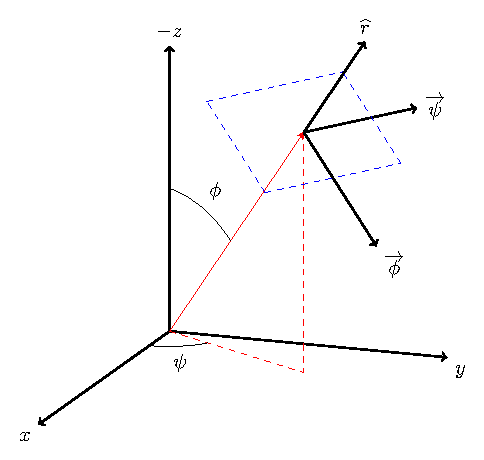
\includepdf{./illustration/repereSiCP.pdf}

\begin{center}
	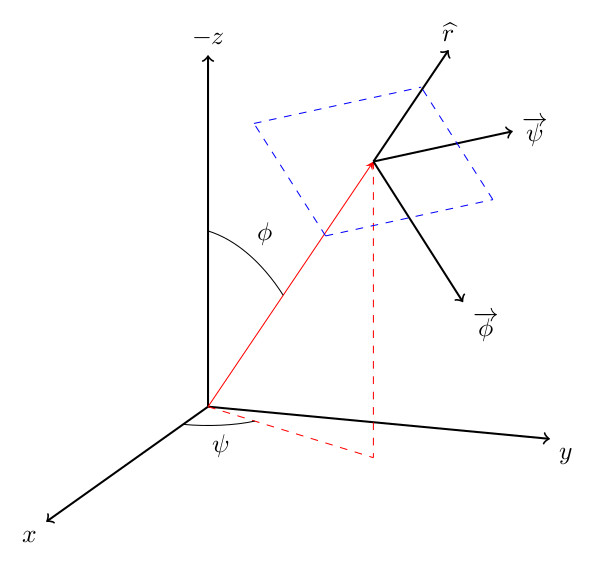
\includegraphics[scale=.97]{./illustration/repereSiCP}
\end{center}

	$\overrightarrow{r}  = \text{} .
	\begin{pmatrix}
		\cos \psi . \sin \phi \\
		\sin \psi . \sin \phi \\
		\cos \phi
	\end{pmatrix}$,

	$\overrightarrow{\psi} = \text{largeur} .
	\begin{pmatrix}
		- \sin \psi \\
		\cos \psi \\
		0
	\end{pmatrix}$,

	$\overrightarrow{\phi} = \text{hauteur} .
	\begin{pmatrix}
		- \cos \psi . \cos \phi \\
		- \sin \psi . \cos \phi \\
		\sin \phi
	\end{pmatrix}$.
%
\subsection{Mathématique}
\begin{description}[leftmargin=0.1cm, itemsep=5pt]
\item{\bf System} : $\theta _\text{i}$.
\item{\bf Chaine} : {\bf r}$_\text{i}$.
\item{\bf Support} : {\bf R}$_\text{i}$.
\item{\bf Point de vue} : {\bf M}, {\bf i}$_\text{M}$,
                                   {\bf j}$_\text{M}$,
                                   {\bf k}$_\text{M}$.
\end{description}
\subsection{Classes}
\begin{description}[leftmargin=0.1cm, itemsep=5pt]
\item{\bf System} : nouveau[N].
\item{\bf Chaine} : chaine[N], support[12], largeur, hauteur.
\item{\bf Point de vue} : perspective, distance, psi, phi.
\end{description}
\subsection{Projection}
\begin{description}[leftmargin=0.1cm, itemsep=5pt]
\item{\bf System-Chaine} : r$_\text{i} = 
	\begin{pmatrix}
		\text{largeur} / 2 \text{N} ( \text{i} - \text{N} / 2 ) \\
		\text{hauteur}. \sin \theta _\text{i} \\
		\text{hauteur}. \cos \theta _\text{i}
	\end{pmatrix}$.
\item{\bf Point de vue} : 
	$\overrightarrow{r}  = \text{} .
	\begin{pmatrix}
		\cos \psi . \sin \phi \\
		\sin \psi . \sin \phi \\
		\cos \phi
	\end{pmatrix}$,
	$\overrightarrow{\psi} = \text{largeur} .
	\begin{pmatrix}
		- \sin \psi \\
		\cos \psi \\
		0
	\end{pmatrix}$,
	$\overrightarrow{\phi} = \text{hauteur} .
	\begin{pmatrix}
		- \cos \psi . \cos \phi \\
		- \sin \psi . \cos \phi \\
		\sin \phi
	\end{pmatrix}$.
\item{\bf Chaine-Rendu} : $\text{g}_\text{i} = 
	\begin{pmatrix}
	(\text{\bf r}_\text{i} - \text{\bf M}).{\text{\bf k}}_\text{M} + \text{hauteur} / 2 \\
	(\text{\bf r}_\text{i} - \text{\bf M}).{\text{\bf j}}_\text{M} + \text{largeur} / 2
	\end{pmatrix}$.
\end{description}
%%%%%%%%%%%%%%%%%%%%%%%%%%%%%%%%%%%%%%%%%%%%%%%%%%%%%%%%%%%%%%%%%%%%%%%%%%%%%%%%%%%%%



%%%%%%%%%%%%%%%%%%%%%
\section{Transformée de fourier rapide}
%%%%%%%%%%%%%%%%%%%%%
Cette section traite de la numérisation de la transformée de fourier grâce aux algorithmes DFT et FFT. \cite{dft-fft}
%%%%%%%%%%%%%%%%%%%%%%%%%%%%%%%%%%%%%%%%%%%%%%%%%%%%%%%%%%%%%%%%%%%%%%%%%%%%%%%%%%%%%

%
%%%%%%%%%%%%%%%%%%%%%%%%%%%%%%%%%%%%%%%%%%%%%%%%%%%%%%%%%%%%%%%%%%%%%%%%%%%%%%%%%%%%

%
\chapter{Développement}

Ce chapitre traite de la structure et du développement des programmes de simulation.

%
%%%%%%%%%%%%%%%%%%%%%
\section{Langage et librairies}
%%%%%%%%%%%%%%%%%%%%%
%
%
\subsection{C}
%
Les progammes SiCP, SiCF et SiGP sont écrit en C \cite{guide-C} \cite{langage-C} et utilisent la librairie SDL.
%
\subsection{SDL 1.2}
%
L'utilisation de la librairie SDL permet la réalisation d'une interface graphique et dynamique avec l'utilisateur.
%
\subsection{SDL 2}
%
Les progammes SiCP, SiCF et SiGP ont évolués vers les progammes SiCP2, SiCF2 et SiGP2 utilisant la version 2
de la librairie SDL.
%
%
%%%%%%%%%%%%%%%%%%%%%%%%%%%%%%%%%%%%%%%%%%%%%%%%%%%%%%%%%%%%%%%%%%%

%
%%%%%%%%%%%%%%%%%%%%%
\section{Modèle Vue Controleur}
%%%%%%%%%%%%%%%%%%%%%
%
%
\subsection{Les répertoires des simulateurs}
\begin{itemize}[leftmargin=2cm]
\item \texttt{donnees} : Inclusion des librairies, constantes et valeurs initiales du système et du graphisme
\item \texttt{fonctions} : Outils mathématique. Fonctions et projection du système
\item \texttt{modele} : Système simulé. 
\item \texttt{graphisme} : Représentation graphique et affichage
\item \texttt{controle} : Liaison entre le système et l'interface graphique 
\item \texttt{objet} : Répertoire pour la compilation
\end{itemize}
%
\subsection{Le modèle}
Le système est un ensemble de pendules couplés
%
\subsection{La vue}
Construit une représentation graphique du système et affiche celle-ci.
%
\subsection{Le controleur}
Exécute alternativement la vue et le modèle. Exécute les actions du clavier.
%
%%%%%%%%%%%%%%%%%%%%%%%%%%%%%%%%%%%%%%%%%%%%%%%%%%%%%%%%%%%%%%%%%%%

%
%%%%%%%%%%%%%%%%%%%%%
\section{Diagrammes}
%%%%%%%%%%%%%%%%%%%%%
%
\subsection{Cas d'utilisation}
%
\subsection{diagramme de classe}
%

%%%%%%%%%%%%%%%%%%%%%%%%%%%%%%%%%%%%%%%%%%%%
%%%%%%%%%%%%%%%%%%%%%%%%%%%%%%%%%%%%%%%%%%%%
\begin{itemize}[leftmargin=2cm]
\item \texttt{gras} : texte
\end{itemize}



%%%%%%%%%%%%%%%%%%%%%%%%%%%%%%%%%%%%%%%%%%%%%%%%%%%%%%%%%%%%%%%%%%%%%%%%%%%%%%%%%%%%%

%
%%%%%%%%%%%%%%%%%%%%%
\section{Evolution}
%%%%%%%%%%%%%%%%%%%%%
%
%
\subsection{La branche ted}
Acronyme de "toujours en dévelopement" la version ted des simulateurs teste les dernieres évolutions.
%
\subsection{Sensibilité aux conditions initiales}
Le controleur actuel des simulateurs possède un unique système. Un second système devrait lui être attribué afin d'observer simultanément l'évolution de deux systèmes et d'observer ainsi la sensibilité aux conditions initiales.
%
%%%%%%%%%%%%%%%%%%%%%%%%%%%%%%%%%%%%%%%%%%%%%%%%%%%%%%%%%%%%%%%%%%%

%
%%%%%%%%%%%%%%%%%%%%%
\section{Valeurs implicites}
%%%%%%%%%%%%%%%%%%%%%
%
%
\subsection{Réglage de dt, durée et pause}
Une incrémentation du système correspond à une avancée dans le temps de \texttt{dt}. La longueur des pendules est fixé à 25 cm afin de battre la seconde :
Période égale à une seconde
\begin{center}
	\begin{tabular}{rcccl}
	T & = & 2$\pi \sqrt{l/g}$ & = & 1\\
	g/l & = & 4$\pi^2$ & = & 39,478\\
	l & = & 0,25 cm &\\
	\end{tabular}
\end{center}
Empiriquement, un affichage graphique par 30 ms, est obtenue avec une pause de l'ordre de 25ms. Si à chaque affichage correspond à une centaine d'incrémentation de dt, 
\begin{center}
	\begin{tabular}{rcl}
	dt $\times$ duree & = & delay\\
	dt $\times$ 100 & = & 0,03\\
	dt & = & 0,0003\\
	\end{tabular}
\end{center}
La valeur de\texttt {duree} peut être changée dynamiquement avec les touches \texttt{F11} et \texttt{F12} afin de faire varier la vitese de la simulation. La valeur de dt peut être réglée avec l'option \texttt{dt} au démarrage du programme, celle de delay par l'option \texttt{pause}.
Dans SiCP, les valeurs implicites de \texttt{dt} et \texttt{duree} sont égale à 0,0003 et 91, celle de pause est égale à 25. Ces valeurs peuvent être affinée suivant le microprcesseur afin d'avoir un pendule qui bat la seconde.
%
%
\subsection{Limite infinie}
La touche \texttt{v} supprime les frottements sauf pour les derniers pour lesquels les frottements s'accroissent. Ceci permet d'obtenir une extrémité "absorbante".
\begin{itemize}[label=\ding{32}, leftmargin=2cm]
\item pendule de  « précédent »  à  «  nombre $\times$ 5 / 6 » : dissipation de 10 à 1,
\item pendule précédents : dissipation = 0,0
\end{itemize}
%
%
\subsection{dt et dissipation maximale}
La touche \texttt{v} supprime les frottements sauf pour les derniers pour lesquels les frottements s'accroissent. Ceci permet d'obtenir une extrémité "absorbante".
\begin{center}
	\begin{tabular}{rcl}
	dt $\times$ DISSIPATION\_MAX & = & constante\\
	0.0003 $\times$ 333 & = & 0,0999\\
	dissipation maximale & = & 0,0999/dt\\
	\end{tabular}
\end{center}
%
%
\subsection{Limitation des valeurs des variables}
%
\subsubsection{Paramètres physiques}
%
Au delà de certaines valeurs de certain paramètres dynamiques, la simulation s'éloigne du comportement physique.
%
\begin{itemize}[label=\ding{32}, leftmargin=2cm]
\item Pour des raisons de discrétisation
\item En raisons de possibles erreurs d'algorithme
\item En raisons de possibles erreurs d'écriture
\end{itemize}
%
Aussi, le fichier \texttt{donnees/constantes.c} contient des valeurs maximale et minimale de certains paramètres. Ces bornes permettent de consolider le comportement des programmes.

En particulier, dans le calcul de la représentation du graphe de SiCP, les coordonées polaires du point de vue sont bornées, $\phi$ ne peut pas être égale à zéro, sa valeur minimale est égale à \texttt{EPSILON} afin d'éviter un plantage due à l'algorithme simplifiée de la représentation graphique.
%
\subsubsection{Paramètres dynamiques}
%
\begin{itemize}[label=\ding{32}, leftmargin=2cm]
\item Vitesse des mobiles
\item Distance entre les mobiles
\item Énergie
\end{itemize}
%
Actuellement, l'angle des pendules de SiCP est borné grâce à une fonction de jauge ramenant la position du premier pendule entre -$\pi$ et $\pi$.
Un test sur la valeur de l'énergie et la limitation de celle-ci permetrait sans doute de consolider davantage le programme. En effet, parmi les bug connus, une valeur trop grande des variables apparait en premier lieu dans la valeur de l'énergie totale.

Ainsi, afin de limiter la vitesse des mobiles, la position des mobiles pourrait être divisées par deux dans les équations linéaires lorsque l'énergie totale est supérieur à \texttt{ENERGIE\_SECURITE}.
%\subsubsection{Énergie maximale}
%La valeur de l'énergie permetrait de limiter un certain nombres d'erreurs.
%
%Lorsque l'énergie est supérieur à ENERGIE\_SECURITE, La position des mobiles pourrait être divisées par deux dans les équations linéaires
%\begin{center}
%	\begin{tabular}{rcl}
% &  &1 009 200 790 976 791 136 174 080\\
% &  &  585 891 747 701 731 153 149 952\\
%      999000555444333222111\\
%\multicolumn{3}{c}{\#define ENERGIE\_SECURITE 777666555444333222111}\\
%	\end{tabular}
%\end{center}
%

%%%%%%%%%%%%%%%%%%%%%%%%%%%%%%%%%%%%%%%%%%%%%%%%%%%%%%%%%%%%%%%%%

%
%
%====================== INCLUSION DE LA BIBLIOGRAPHIE ======================
%
%récupérer les citation avec "/footnotemark"
%\nocite{*}
%choix du style de la biblio
\bibliographystyle{plain}
%inclusion de la biblio
\cleardoublepage
\addcontentsline{toc}{chapter}{Bibliographie}
\bibliography{bibliographie.bib}
%\newpage
%\input{./glossaire/glossaire.tex}
%\newpage
%\input{./annexes/annexes.tex}
\end{document}
%%%%%%%%%%%%%%%%%%%%%%%%%%%%%%%%%%%%%%%%%%%%%%%%%%%%%%%%%%%%%%%%%%%%%%%%%%%%%%%%%
